\documentclass[11pt,a4paper]{article}
\usepackage[margin=2.5cm]{geometry}
\usepackage{enumitem}
\setlist{itemsep=1pt,topsep=3pt}
\usepackage{caption}
\captionsetup{font=small,labelfont=bf}

\usepackage{amsmath,amssymb}
\usepackage{graphicx}
\usepackage{booktabs}
\usepackage{multirow}
\usepackage{array}
\usepackage{tabularx}
\usepackage[dvipsnames]{xcolor}
\usepackage{tikz}
\usetikzlibrary{arrows.meta,positioning,fit}
\usepackage{url}
\usepackage[hidelinks]{hyperref}
\usepackage{cite}

\newcommand{\code}[1]{\texttt{#1}}
\newcommand{\est}{\textsc{est}}   % established stations 1--3
\newcommand{\ho}{\textsc{ho}}     % held-out station 4

\begin{document}

\title{Inductive Bias versus Flexibility in Multi-Horizon Forecasting:\\ From Period-Routed Ridge to Autoformer}

\author{Mubeen Ahmed\\[2pt]
\small Department of Artificial Intelligence, School of Science and Engineering\\
\small Lahore University of Management Sciences, Lahore, Pakistan\\
\small Roll no.\ 25280101 \quad \texttt{25280101@lums.edu.pk}\\[4pt]
\small AI651 Deep Learning for Space, Time and Graphs, Programming Assignment 1, Fall 2026\\
\small Code: \url{https://github.com/mubeenahmed-ai/AI651-PA1-Forecasting}}
\date{}

\maketitle

%=====================================================================
\begin{abstract}
We study how much a well-chosen inductive bias matters, compared with model flexibility, in multi-horizon time-series forecasting. We do so in two settings.

\emph{Task 1} is a simulated four-station vibration line whose operating pace changes between runs. On it we compare fixed, sensor-specific and period-routed ridge maps with Attention forecasters extended by moving-average decomposition and FFT-based delay mixing. A period-routed linear map, which is given the one variable that changes the correct continuation, attains the lowest validation error on both established and held-out stations (MSE 0.028 and 0.030\,(m/s$^2$)$^2$), with $6\times$ fewer parameters than any neural model. Decomposition and delay mixing each help Attention, but their gains are sub-additive.

\emph{Task 2} forecasts 168 steps of a heavy-tailed real series with an Autoformer. Over 120 multi-seed runs on a chronological split, future-known external variables reduce the mean block RMSE by 18.8 on validation, while past-only covariates give no benefit. A per-horizon diagnosis shows that the reference decoder initialisation ignores the most recent level. A one-parameter learned decay initialisation halves the one-step error and improves validation RMSE on every seed. The submitted 6{,}626-parameter model scores RMSE 101.1 on the hidden week.

In both settings, simple models with the right structure match or beat flexible ones.
\end{abstract}

\noindent\textbf{Keywords:} time-series forecasting, inductive bias, series decomposition, auto-correlation, Autoformer, ridge regression

%=====================================================================
\section{Introduction}
A forecaster must decide how much structure to assume. Linear maps assume a fixed relation between past and future. Attention~\cite{vaswani2017} lets each context build its own mixing rule. Autoformer~\cite{wu2021} assumes that series separate into trend and seasonal parts, and that dependencies are organised by periodic delays. Stronger assumptions make learning easier when they hold and harmful when they do not. Recent work shows that simple linear models often rival Transformer forecasters~\cite{zeng2023}.

This report answers one question in two settings: \emph{how much does the right inductive bias matter compared with a more flexible model?}

\textbf{Contributions.}
\begin{enumerate}
  \item \textbf{Synthetic benchmark (Task~1).} We implement Raw Attention, centred moving-average decomposition, and delay aggregation. We show that period routing, a hand-supplied bias, beats every learned mixer on both populations, and that the two architectural upgrades overlap. The ranking is stable across three model seeds.
  \item \textbf{Real series (Task~2).} We build an Autoformer from its two defining mechanisms. A 120-run, multi-seed validation study establishes which external variables help, and when their values must be available for them to help.
  \item \textbf{Decoder initialisation.} We identify a failure of the reference decoder initialisation at short horizons and correct it with a one-parameter learned decay, grounded in the optimal forecast of a short-memory process.
  \item \textbf{Code audit.} We audit the supplied harness and report the caveats that affect interpretation.
\end{enumerate}
All code, run logs and figures are in the public repository listed above.

%=====================================================================
\section{Background and Related Work}
\textbf{Linear forecasting.} Ridge regression fits one map $\widehat W=(X^\top X/n+\lambda I)^{-1}X^\top Z/n$ from contexts $X$ to targets $Z$. A sinusoid of known period obeys an exact linear recurrence, so a linear map can continue it perfectly. It needs a different map for each period, however.

\textbf{Attention.} Attention~\cite{vaswani2017} computes $\mathrm{softmax}(QK^\top/\sqrt{d_h})V$ with $Q,K,V$ projected from the input. The projections are fixed after training, but the weights are recomputed per context, and every one of the $L^2$ position pairs is scored separately.

\textbf{Decomposition.} Classical pipelines separate trend and seasonality once, e.g.\ by moving averages or STL~\cite{cleveland1990,hyndman}. Autoformer~\cite{wu2021} instead decomposes progressively inside every layer. A centred average of width $m$ passes a fraction
\begin{equation}
|G_m(P)|=\left|\frac{\sin(\pi m/P)}{m\,\sin(\pi/P)}\right|
\label{eq:gain}
\end{equation}
of a period-$P$ cycle into its trend.

\textbf{Auto-Correlation.} Autoformer replaces point-wise attention by scoring delays, $R(\tau)=\sum_t q_t k_{(t-\tau)\bmod L}$, which the FFT computes in $O(L\log L)$. It then aggregates values from the top-$k$ delays. For a sinusoid, $R(\tau)\propto\cos(2\pi\tau/P)$.

%=====================================================================
\section{Task 1: Problem Setup}
\textbf{Data.} Four accelerometers (20\,Hz, 15{,}360 samples each) record
\[
y_i(t)=b_i(t)+s_i(t)+\epsilon_i(t),
\]
i.e.\ a slow drift, a vibration, and noise with $\sigma=0.09$.
\begin{itemize}
  \item \textbf{Products.} Products A, B, C alternate every 192 samples. Each run has one vibration period, drawn from its product's range (14--18, 21--27, 28--36 samples) and shared by all stations.
  \item \textbf{Drift.} The drift has period 240. Over one context it spans up to 9.1\,m/s$^2$, against 3.5 for the vibration.
  \item \textbf{Populations.} Stations 1--3 are \emph{established} (\est). Station~4 is \emph{held out} (\ho): it is never used for fitting.
\end{itemize}

\textbf{Protocol.}
\begin{itemize}
  \item Context $L=96$, horizon $H=48$. No window crosses a changeover.
  \item Targets lie in train $[0,9600)$, validation $[9600,12480)$ and test $[12480,15360)$.
  \item Each context is anchored at its last value $a$ and divided by one training scale $c$; forecasts are $\hat y=a+c\hat z$.
  \item All results come from one fresh \code{PA1\_PRESET=full} run (data and model seed 0). Every harness check passed.
  \item Unless stated otherwise, errors are \emph{validation} errors in physical units.
\end{itemize}

%=====================================================================
\section{Task 1: Methods}
\textbf{Linear baselines.} \emph{Shared ridge} fits one $\widehat W$ to all \est{} windows. \emph{Sensor-specific ridge} fits one per established station. \emph{Period-routed ridge} estimates the context's period, snaps it to one of 13 fixed 1.5-sample pace bands, and uses that band's $\widehat W$.

\textbf{Raw Attention (implemented).} A circular 3-tap convolution embeds the context to width $d=64$. A learned position table is added, followed by two pre-norm encoder blocks (Attention and feed-forward, with residual connections), a LayerNorm, flattening, and a linear head to $H$ outputs: 368{,}368 parameters.

\textbf{Series decomposition (implemented).} For odd width $m=2q+1$, the trend is
\[
T_t=\frac{1}{m}\sum_{u=-q}^{q}x_{t+u},
\]
computed after replicating the first and last samples $q$ times. We return $(S,T)=(x-T,T)$, which makes $S+T=x$ exact. The decomposed forecaster sends $S$ to the encoder and $T$ to a linear trend head, adds the two forecasts, and re-decomposes after every residual sub-layer.

\textbf{Delay mixer (aggregation implemented).} Scores $R(\tau)$ are computed on projected $q,k$ (supplied). Delays are restricted to $\{8,\dots,48\}$, and the top $K=\lceil2\ln96\rceil=10$ are kept with weights $\alpha_j=\mathrm{softmax}_j(R(\tau_j)/\vartheta)$ at a learned temperature $\vartheta$. We implement
\begin{equation}
z_t=\sum_{j=1}^{K}\alpha_j\,v_{(t-\tau_j)\bmod L}
\label{eq:agg}
\end{equation}
as a per-example gather along time. Delays and weights are shared across heads and features, and the operation is differentiable in both $v$ and $\alpha$. On the worked example ($v=[10,20,30,40]$, delays $[1,3]$, weights $[\frac34,\frac14]$) it returns $[35,15,25,25]$, which confirms the shift direction.

\textbf{2$\times$2 design.} A single network toggles two switches: representation (raw or decomposed) and mixer (Attention or delay). This gives Raw Attention, Attention + decomposition, Raw delay mixer, and Autoformer-inspired. An audit (Section~\ref{sec:audit}) verified that the Part~1/2 classes are bit-identical to the unified network at matching settings, so the comparison changes only the switches.

%=====================================================================
\section{Task 1: Results}

\begin{table}[htbp]\centering\small
\caption{Validation errors (Outputs 1.1 and 4.1). RMSE in m/s$^2$, MSE in (m/s$^2$)$^2$. \est{} = Stations 1--3; \ho{} = held-out Station~4. Fit time on CPU.}
\label{tab:t1}
\resizebox{\linewidth}{!}{%
\begin{tabular}{lcccccccrr}
\toprule
& \multicolumn{5}{c}{\est} & \multicolumn{2}{c}{\ho} & & \\
\cmidrule(lr){2-6}\cmidrule(lr){7-8}
Model & RMSE & MSE & A & B & C & RMSE & MSE & Params & Fit (s)\\
\midrule
Shared ridge & 0.767 & 0.588 & 0.805 & 0.854 & 0.621 & 0.876 & 0.767 & 4{,}608 & $<$0.01\\
Sensor-specific ridge & 0.768 & 0.590 & 0.804 & 0.852 & 0.630 & n/a & n/a & 13{,}824 & $<$0.01\\
Period-routed ridge & \textbf{0.166} & \textbf{0.028} & 0.181 & 0.164 & 0.152 & \textbf{0.173} & \textbf{0.030} & 59{,}904 & $<$0.01\\
\midrule
Raw Attention & 0.424 & 0.180 & 0.387 & 0.463 & 0.419 & 0.621 & 0.385 & 368{,}368 & 707\\
Attention + decomposition & 0.299 & 0.089 & 0.268 & 0.341 & 0.282 & 0.444 & 0.197 & 373{,}024 & 745\\
Raw delay mixer & 0.217 & 0.047 & 0.208 & 0.207 & 0.234 & 0.340 & 0.116 & 368{,}370 & 736\\
Autoformer-inspired & 0.199 & 0.039 & 0.223 & 0.189 & 0.182 & 0.240 & 0.058 & 373{,}026 & 758\\
\bottomrule
\end{tabular}}
\end{table}

\subsection{Context-dependent forecasting (Responses 1A, 1B)}
\textbf{Response 1A (expected ordering).} We derived an expected ordering from each model's assumptions as the handout describes them:
\begin{itemize}
  \item \est: period-routed $<$ Raw Attention $<$ shared $\approx$ sensor-specific. Routing supplies the variable that changes the rule; Attention adapts but must learn how; one fixed map must compromise across paces; station identity carries no pace information.
  \item \ho: the same order without sensor-specific ridge, with some degradation for every model and most for the neural one.
\end{itemize}

\textbf{Response 1A (measured, Table~\ref{tab:t1}).}
\begin{itemize}
  \item \est: period-routed (0.166) $<$ Raw Attention (0.424) $<$ shared (0.767) $\approx$ sensor-specific (0.768).
  \item \ho: 0.173 $<$ 0.621 $<$ 0.876.
  \item \textbf{Magnitudes.} Routing cuts shared-ridge RMSE by 78\% and beats Raw Attention by $2.6\times$ on \est. From \est{} to \ho, Raw Attention degrades by 46\%, against only 4\% for routed ridge.
  \item \textbf{Products.} Shared ridge is worst on Product~B (0.854) and best on C (0.621). Routed ridge is flat (0.152--0.181).
\end{itemize}

\textbf{Response 1A (revision).} The ordering was confirmed, but two magnitudes were revised upward. The first is routing's margin over Attention. The second is Attention's held-out loss. That loss exceeds pure amplitude scaling: anchored linear maps are scale-equivariant, and shared ridge follows amplitude exactly (0.731 on Station~1 at amplitude 1.75, rising to 0.876 on Station~4 at 2.15, against 0.898 predicted). Scaling would put Raw Attention near 0.45 on \ho, yet it is 0.621, which indicates overfitting to three stations.

\textbf{Response 1A (explanation).}
\begin{itemize}
  \item One map must average incompatible phase advances.
  \item Identity is uninformative, because each station runs every pace.
  \item Routing conditions on pace alone, so it transfers to \ho.
  \item Attention adapts per context, but must learn pace and drift from limited data.
\end{itemize}

\begin{figure}[htbp]\centering
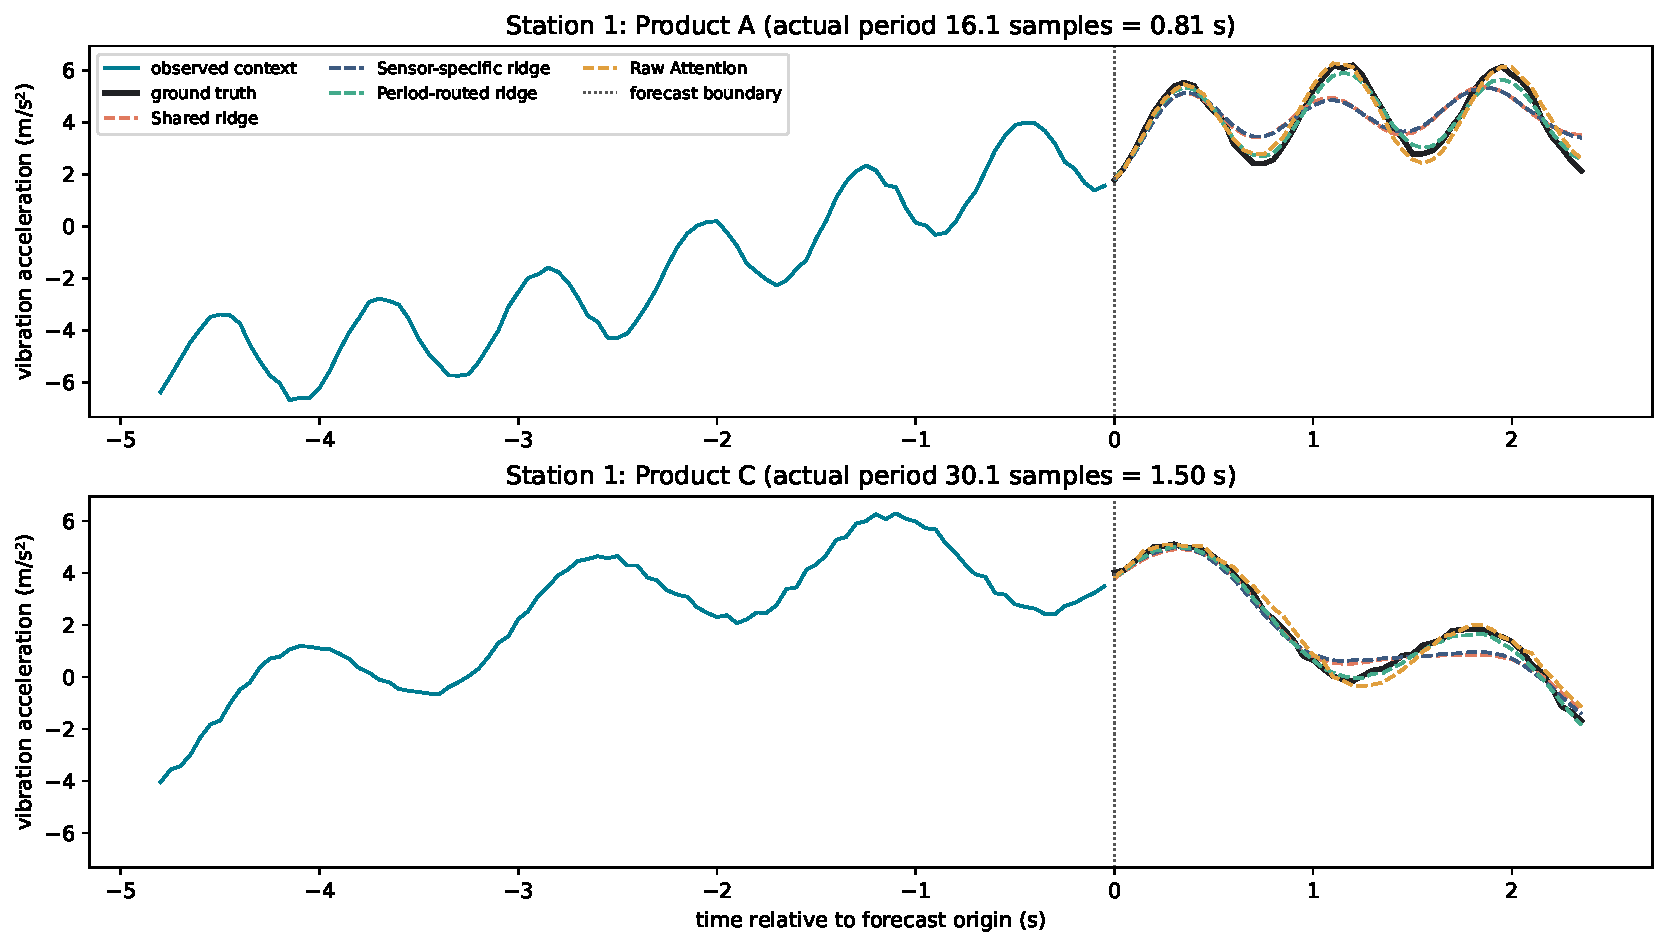
\includegraphics[width=0.88\linewidth]{figures/task1_output_1-2.pdf}\\[4pt]
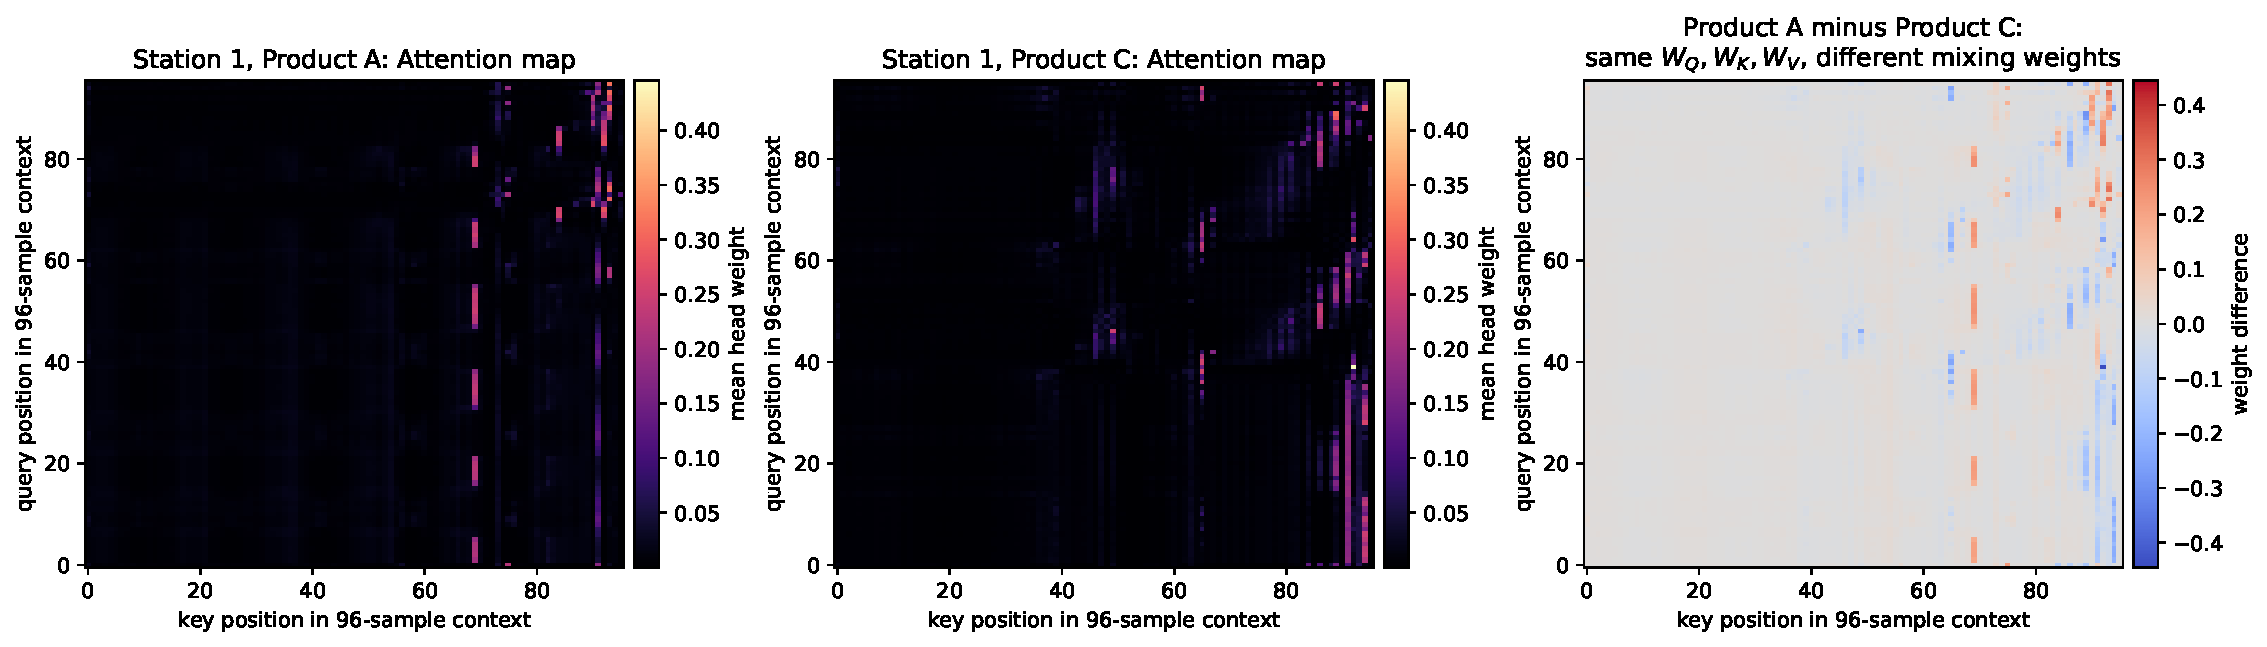
\includegraphics[width=\linewidth]{figures/task1_output_1-3.pdf}
\caption{Top: Output 1.2, Station~1 under Product~A ($P=16.1$) and Product~C ($P=30.1$). Bottom: Output 1.3, first-layer Attention maps for the same station under both products, and their difference.}
\label{fig:t1ctx}
\end{figure}

\textbf{Response 1B.} The correct continuation advances the phase by $2\pi h/P$, so $P\approx16$ and $P\approx30$ require different linear operators. The single least-squares $\widehat W$ of Eq.~(8) in the handout averages them, and an average of phase-shifted sinusoids is a \emph{damped, phase-smeared} sinusoid (Fig.~\ref{fig:t1ctx}, top).
\begin{itemize}
  \item \textbf{Product~A.} Shared ridge's forecast loses amplitude and drifts out of phase: window RMSE 0.779, against 0.232 for routed ridge.
  \item \textbf{Product~C.} The phase error is smaller: 0.448 vs 0.150.
  \item \textbf{Sensor-specific ridge} shows the same shape (0.787, 0.436).
\end{itemize}
In contrast, Attention keeps $W_Q,W_K,W_V$ fixed but recomputes $QK^\top$ from each window. The two contexts therefore yield different mixing operators without refitting: mean $|\Delta|=0.011$, comparable to the uniform weight $1/96$, and max $0.445$ (Fig.~\ref{fig:t1ctx}, bottom). This shows only that the mixing depends on the input, not that Attention has recovered the period.

\subsection{Separating slow structure (Response 2)}
\textbf{Selected width.} We selected $m=41$.
\begin{itemize}
  \item \textbf{Oracle recovery} (training, \est; Output 2.2) rises from 0.687 on the raw context to 0.980, 0.989, 0.993 and 0.998 for $m=17,25,33,41$.
  \item \textbf{Visually} (Output 2.1, Fig.~\ref{fig:t1decomp}), narrow widths let the trend follow the vibration: at $m=17$ the residual std is 0.58, against 1.57 at $m=41$. After decomposition, the periodogram peaks sharply at the true $P=32$.
  \item \textbf{Empirically} (Output 2.3), Attention + decomposition halves Raw Attention's validation MSE: 0.180$\to$0.089 on \est, 0.385$\to$0.197 on \ho, and lower on every product.
\end{itemize}

\textbf{Why the bias fits.} The drift (period 240) and the vibration (14--36) are separated in frequency. By Eq.~\eqref{eq:gain}, $m=41$ keeps 95\% of the drift in $T$ while leaking on average 14\% of the vibration. At $m=17$ the leak is 37\% on average and up to 67\% at $P=36$, matching Fig.~\ref{fig:t1decomp}.

\textbf{The oracle diagnostic.} The oracle measures directly whether a width exposes the repetition, without training one network per width, and it uses training windows only. It saturates, however, and $m=41$ is the largest candidate, so the choice is ``best of four'', not a proven optimum.

\textbf{Failure mode.} An abrupt level shift is smeared over $m$ samples and leaks into $S$. STL~\cite{cleveland1990} would instead assume a locally smooth but curved trend.

\begin{figure}[htbp]\centering
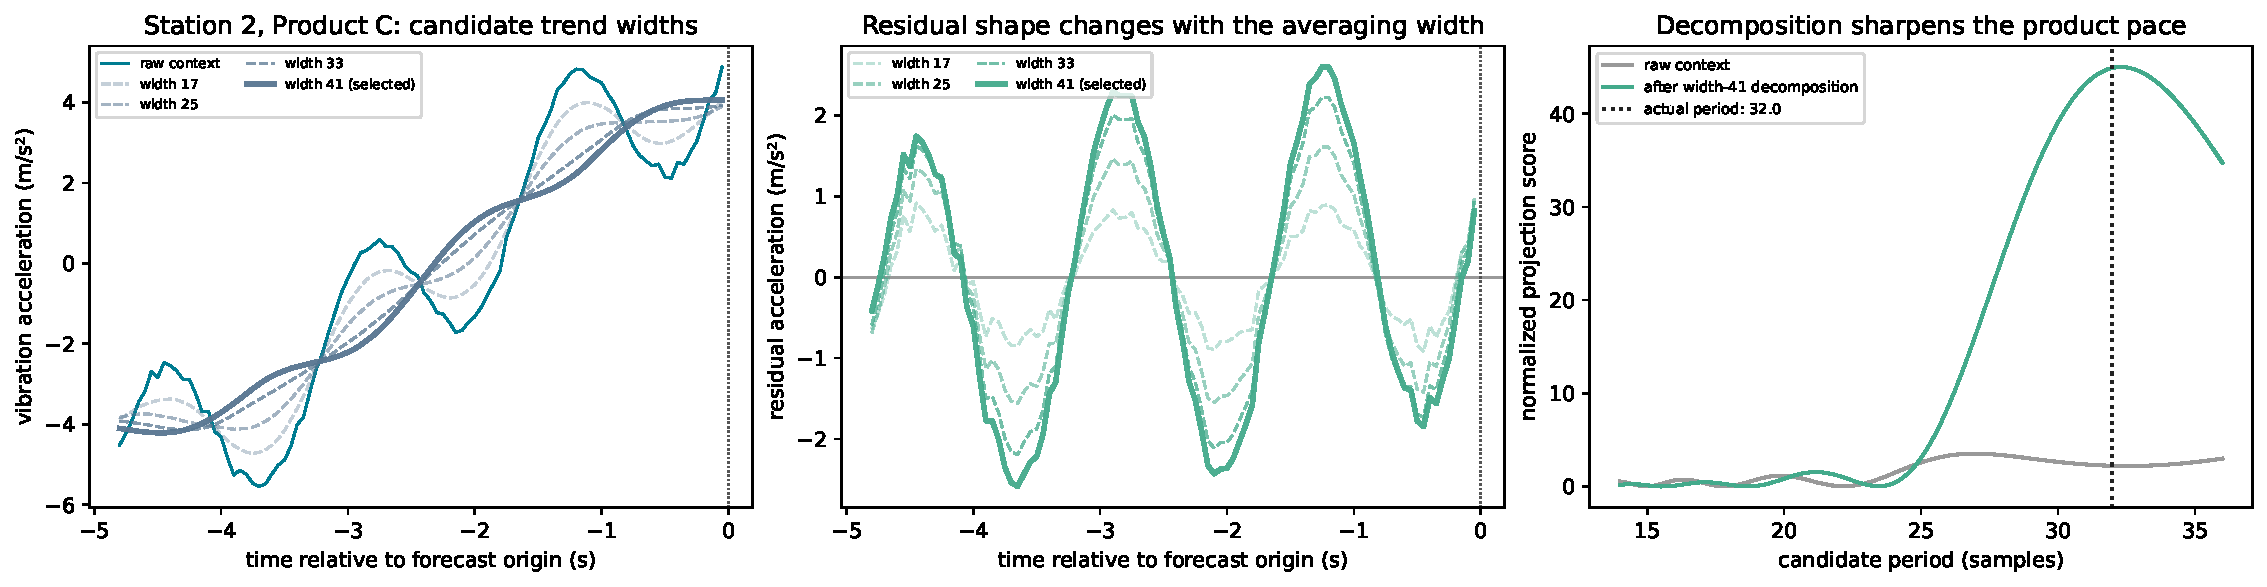
\includegraphics[width=\linewidth]{figures/task1_output_2-1.pdf}\\[4pt]
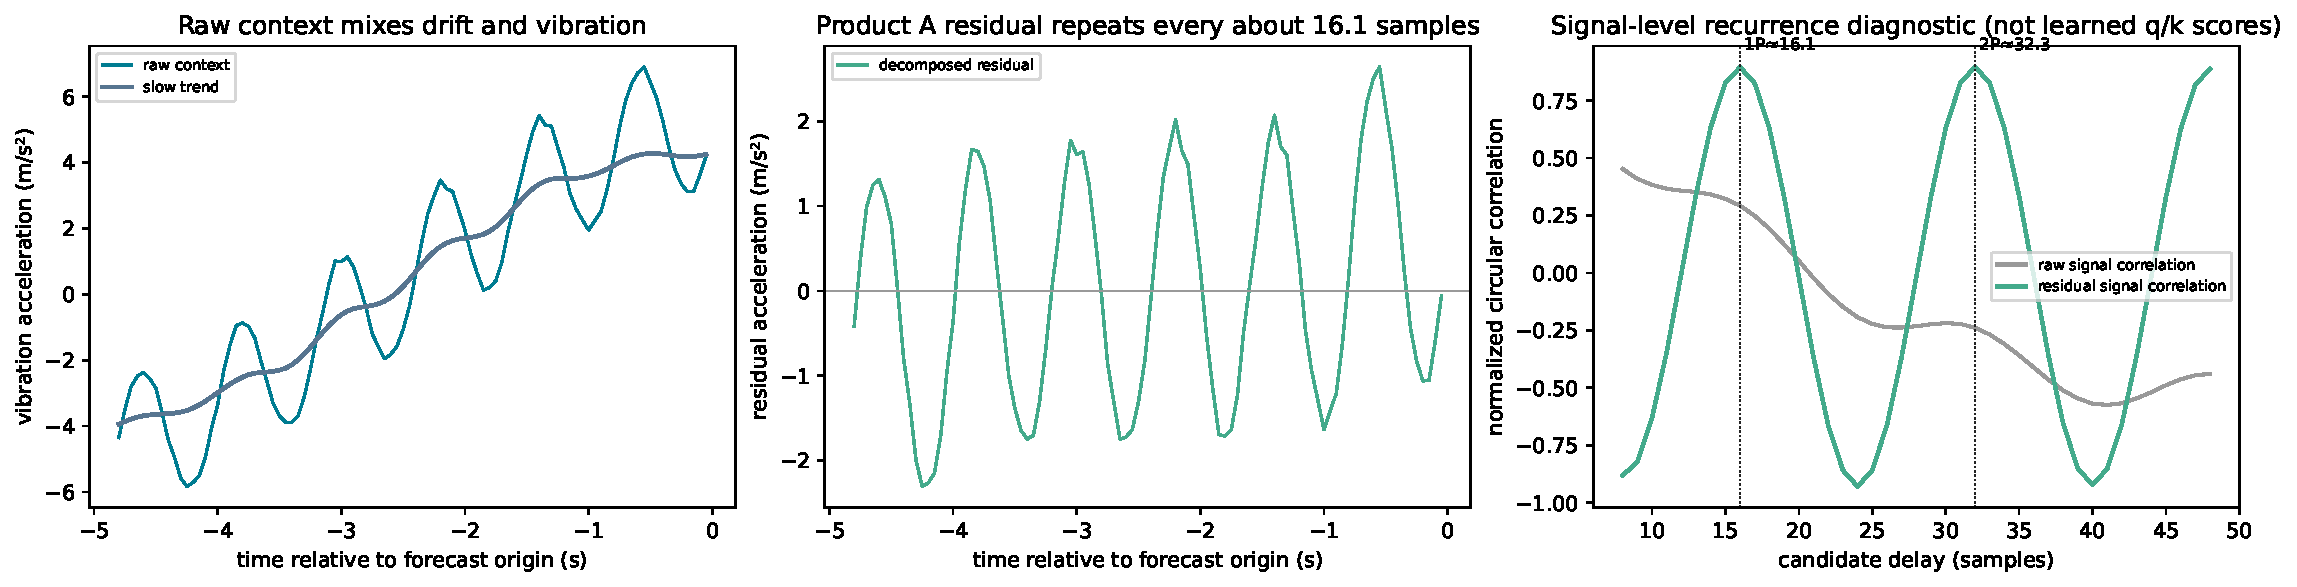
\includegraphics[width=\linewidth]{figures/task1_output_3-2.pdf}
\caption{Top: Output 2.1, candidate trend widths on the validation window with the \emph{largest} raw period error (4.98 samples vs a median of 0.53), i.e.\ a hardest case. Bottom: Output 3.2, signal-level recurrence diagnostic (not learned $q/k$ scores) for a Product~A run with $P=16.13$.}
\label{fig:t1decomp}
\end{figure}

\subsection{Mixing by temporal delay (Response 3)}
\textbf{Implementation.} Eq.~\eqref{eq:agg} passes the worked example and the gradient and axis checks. Output 3.1 confirms that the supplied FFT scores equal the direct circular correlation, $[4,-4,4,-4]$.

\textbf{Strongest lags.} The residual correlation peaks at delays 16 (0.896) and 32 (0.897), the nearest integers to $P=16.13$ and $2P$, with troughs near $P/2$ (Fig.~\ref{fig:t1decomp}, bottom). This is the $\cos(2\pi\tau/P)$ profile expected for a sinusoid. The near-equal peaks reflect $96/P\approx5.95$ cycles fitting the circular ring.

\textbf{Why decomposition helps.} A ramp resembles itself at every shift, so the raw correlation decays smoothly with no peak at $P$. Removing the drift isolates the recurring displacement, supporting a mixer that scores $L$ delays rather than $L^2$ position pairs.

\textbf{Failure mode.} An isolated transient, such as an impact, has no recurring displacement. Delay mixing would then forecast a spurious echo one pseudo-period later. A period drifting within the window fails similarly.

\subsection{Comparing designs and deployment (Response 4)}
\textbf{(a) Prediction} (from the switches' stated assumptions):
\begin{quote}
Decomposition should help most on contexts where the slow component is prominent, because it removes the ramp before the mixer and hands it to a linear trend head. Delay mixing only changes how a still drift-dominated sequence is mixed, and a large ramp makes every delay look alike.
\end{quote}

\begin{figure}[htbp]\centering
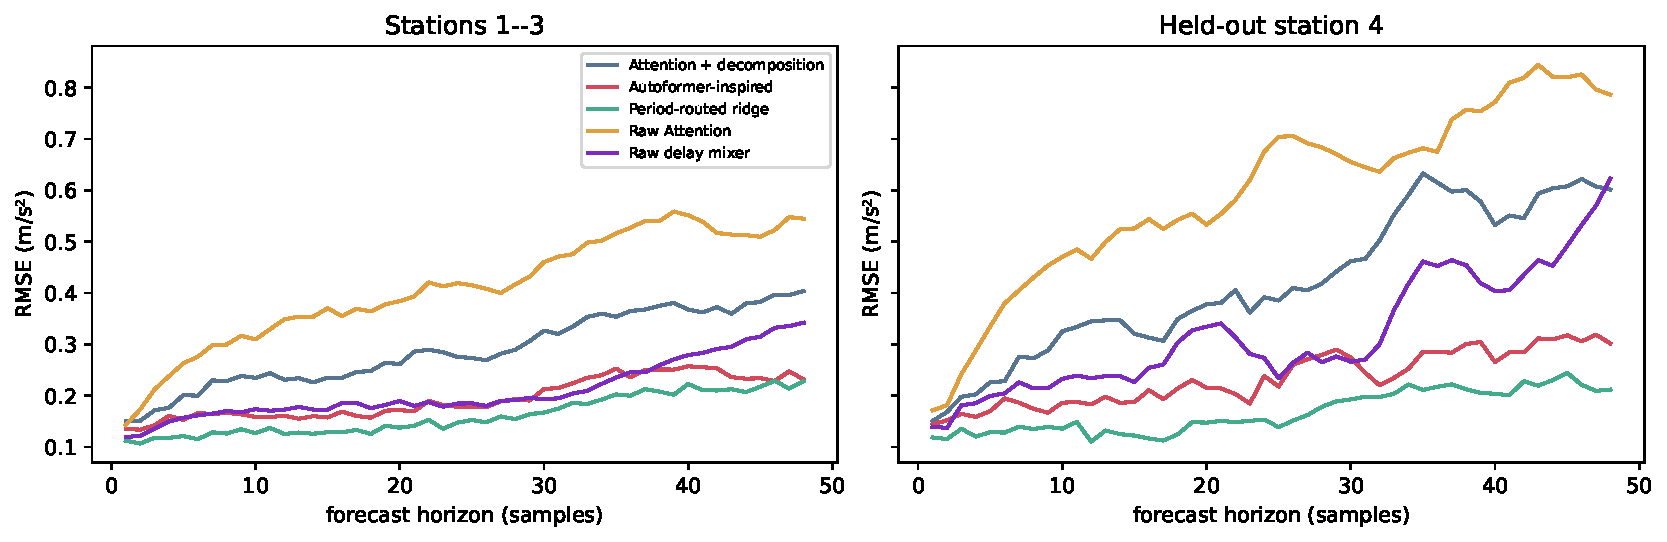
\includegraphics[width=0.85\linewidth]{figures/task1_output_4-2.pdf}
\caption{Output 4.2: validation RMSE along the 48-step horizon, including period-routed ridge.}
\label{fig:t1hor}
\end{figure}

\textbf{(b) Errors.} Validation RMSE and MSE for the four neural models and the linear baselines on \est{} are given in Table~\ref{tab:t1}.

% ---- Response 4 interpretation (<= 200 words; see word-count comment below) ----
\textbf{Interpretation.}
\begin{itemize}
  \item \textbf{Switches (validation MSE gain vs Raw Attention).} \est: decomposition $-0.091$, delay $-0.133$, both $-0.141$ (sum $-0.224$). \ho: $-0.188$, $-0.269$, $-0.327$ (sum $-0.457$).
  \item \textbf{Both help, but the gains overlap} (sub-additive): both target the drift. Delay mixing is the stronger single switch.
  \item \textbf{Horizon (Fig.~\ref{fig:t1hor}).} On \est, error grows along the horizon: Raw Attention 0.14$\to$0.55, Autoformer-inspired 0.14$\to$0.23, period-routed ridge 0.11$\to$0.23.
  \item \textbf{Prediction (a) is not supported.} On the quarter of \est{} validation windows with the largest slow-component range, delay mixing gains $-0.083$ against decomposition's $-0.018$. These windows are near-linear ramps, which anchored models already extrapolate. Decomposition's gain comes from curved-drift windows ($-0.115$).\footnote{Supplementary check: \code{audit/drift\_subgroup\_check.py}.}
\end{itemize}

\textbf{(c) Deployment.} Period-routed ridge for both populations, chosen from the validation-only summary before Output 4.3.
\begin{itemize}
  \item \textbf{Established stations.} Lowest validation MSE (0.028 vs 0.039 for Autoformer-inspired), $6\times$ fewer parameters, and a closed-form fit ($<$0.01\,s vs 758\,s).
  \item \textbf{Held-out Station~4.} Again lowest (0.030 vs 0.058). It routes by estimated pace, not identity, so it needs no Station-4 data.
  \item \textbf{Test (Output 4.3).} RMSE 0.161 (\est) and 0.183 (\ho), matching validation. Model seeds 1--2 give the same ranking.
\end{itemize}
% Word count of the "Interpretation" and "(c)" text above, excluding tables, figures and the footnote: 172 words (<= 200).

\subsection{Robustness}
\textbf{Model seeds.} Retraining the four neural models with seeds 1 and 2 preserves the ranking on both populations. Mean $\pm$ std \est{} validation MSE over seeds 0--2:
\begin{itemize}
  \item Raw Attention $0.192\pm0.012$;
  \item Attention + decomposition $0.071\pm0.017$;
  \item Raw delay mixer $0.042\pm0.006$;
  \item Autoformer-inspired $0.036\pm0.004$;
  \item routed ridge 0.028.
\end{itemize}
Sub-additivity persists: $-0.121$ and $-0.150$ separately, against $-0.156$ combined.

\subsection{Audit of the supplied harness}\label{sec:audit}
\textbf{Verified.} The harness is leakage-safe: scale, $\lambda$ and training all use \est{} training data. No window crosses a changeover, and the $2\times2$ comparison is exact.

\textbf{Caveats for interpretation.}
\begin{enumerate}
  \item Neural checkpoints are selected on the validation split also used for comparison, which slightly favours neural validation scores. Test is unaffected.
  \item The decomposition width is chosen by an oracle, at the edge of its grid.
  \item Output 2.1 plots a worst case.
\end{enumerate}
Eight minor robustness and hygiene issues are documented in \code{audit/CODE\_AUDIT.md}. None alters a reported number.

%=====================================================================
\section{Task 2: Problem and Data}
The task is to forecast $H=168$ steps (time\_idx 43{,}657--43{,}824) of a non-negative series with 43{,}656 released observations.
\begin{itemize}
  \item \textbf{External file.} Ten variables A--J, measured on the same clock, cover the horizon as well. Using their horizon values is permitted.
  \item \textbf{Constraints.} The model must be an Autoformer with progressive series decomposition and Auto-Correlation. Claims require multiple seeds.
  \item \textbf{Score.} Ranking uses RMSE $+\alpha P+\beta E$.
\end{itemize}

\textbf{Exploratory analysis} (training split only).
\begin{itemize}
  \item \textbf{Periodicity.} Without calendar information, the periodogram reveals a 24-step cycle in the target and all continuous covariates, and a $\approx$8{,}766-step cycle, the dominant peak of features A--C (Fig.~\ref{fig:t2eda}). These are the daily and annual cycles of hourly data.
  \item \textbf{Distribution.} The target is heavy-tailed: median 73, mean 98, maximum 994, skew 1.8.
  \item \textbf{Memory.} Autocorrelation is 0.97 at lag~1, 0.40 at lag~24 and $\approx0$ at lag~168. Over a week, a constant training mean therefore beats persistence (validation block RMSE 85.9 vs 105.6).
  \item \textbf{Covariates.} Indicators G--J are one-hot. The strongest covariate links are dew point A (0.67 correlation of 24-step changes), pressure C ($-0.42$) and cumulative wind D ($-0.30$).
\end{itemize}

\begin{figure}[htbp]\centering
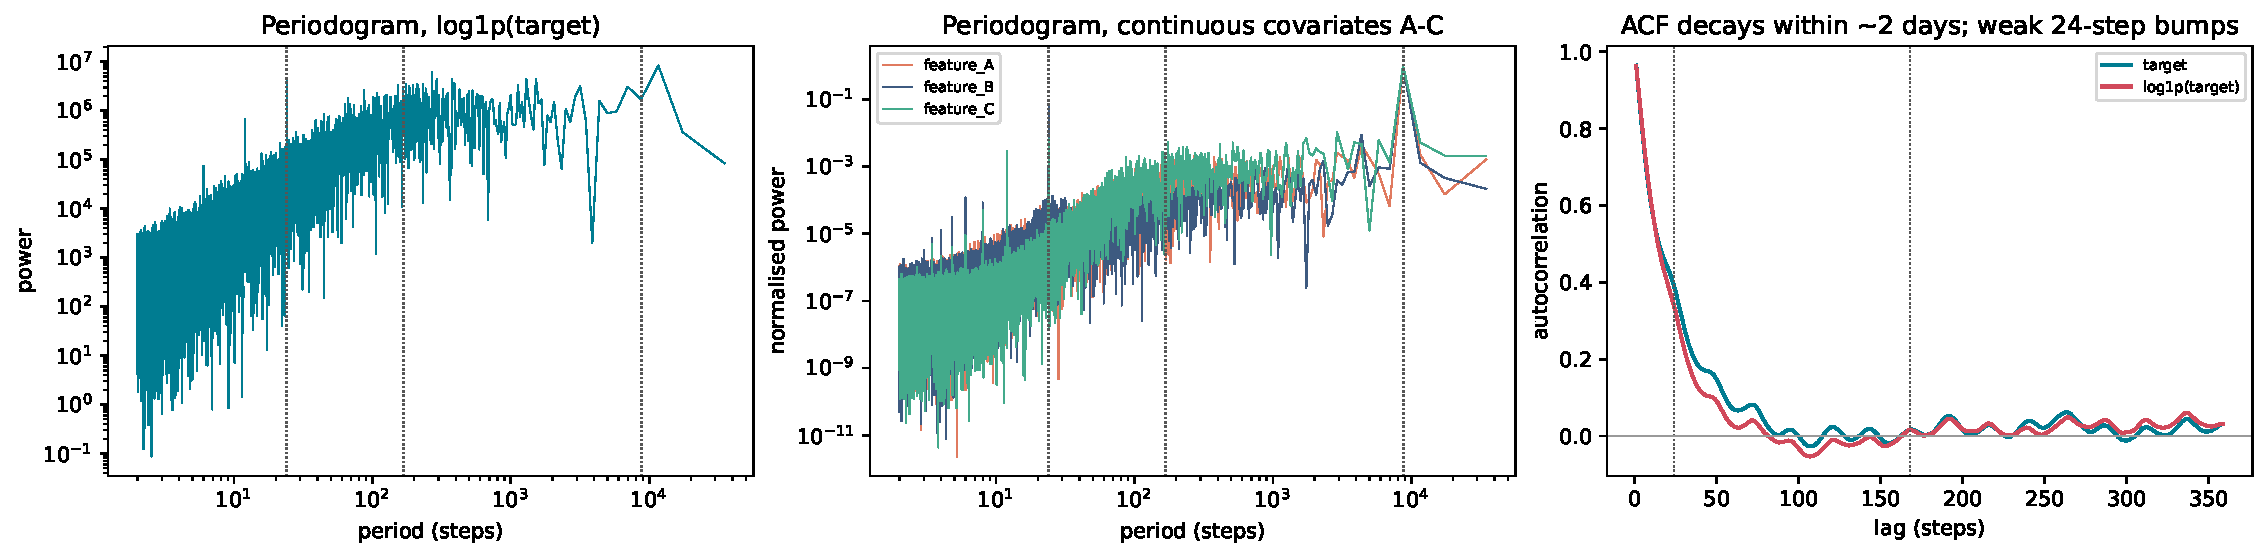
\includegraphics[width=\linewidth]{figures/task2_periodogram.pdf}
\caption{Task 2, training split: periodogram of $\log(1+y)$ and of covariates A--C, and autocorrelation. Dotted lines mark 24, 168 and 8{,}766 steps.}
\label{fig:t2eda}
\end{figure}

%=====================================================================
\section{Task 2: Method}
\textbf{Preprocessing.}
\begin{itemize}
  \item The target is z-scored on the raw scale with training statistics. Forecasts are clipped at 0.
  \item Continuous covariates are z-scored, after $\log(1+\cdot)$ for the heavy-tailed D--F. Indicators stay binary.
  \item Phase features $\sin/\cos(2\pi t/24)$ and $\sin/\cos(2\pi t/8766)$ are computed from the index, so they are known over the horizon.
\end{itemize}

\textbf{Covariate regimes.} These define the ablation:
\begin{itemize}
  \item \emph{future}: the measured horizon values;
  \item \emph{past}: known only to the origin, held at their last value over the horizon;
  \item \emph{none}.
\end{itemize}
Covariates enter as extra \emph{value channels}: in the encoder with the target, and in the decoder with their known future values.

\begin{figure}[htbp]\centering
\resizebox{0.72\linewidth}{!}{%
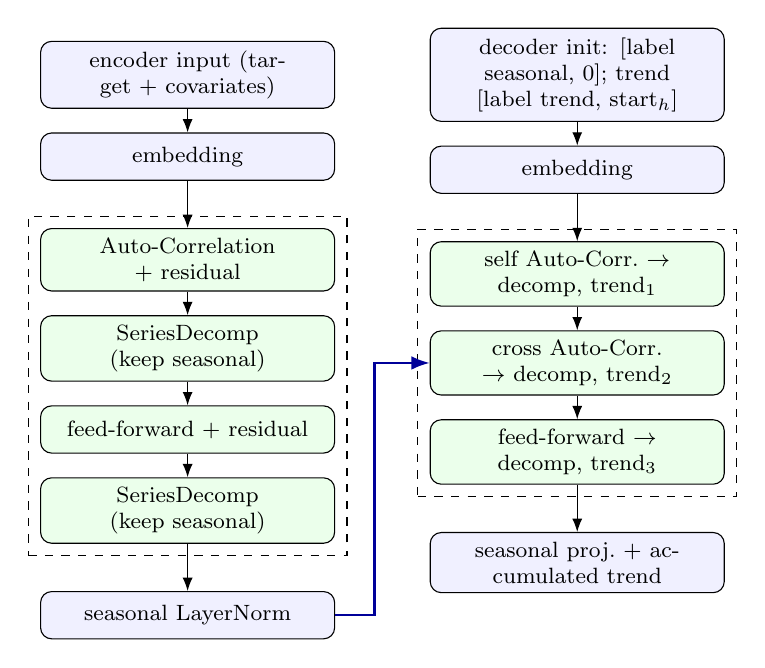
\begin{tikzpicture}[node distance=3mm, every node/.style={font=\footnotesize},
  b/.style={draw,rounded corners,fill=blue!6,align=center,text width=3.5cm,minimum height=6mm},
  g/.style={draw,rounded corners,fill=green!8,align=center,text width=3.5cm,minimum height=6mm}]
\node[b] (xi) {encoder input (target + covariates)};
\node[b,below=of xi] (ee) {embedding};
\node[g,below=6mm of ee] (a1) {Auto-Correlation + residual};
\node[g,below=of a1] (s1) {SeriesDecomp (keep seasonal)};
\node[g,below=of s1] (f1) {feed-forward + residual};
\node[g,below=of f1] (s2) {SeriesDecomp (keep seasonal)};
\node[b,below=6mm of s2] (en) {seasonal LayerNorm};
\node[draw,dashed,fit=(a1)(s2),inner sep=1.5mm] {};
\node[b,right=1.2cm of xi] (di) {decoder init: [label seasonal, 0]; trend [label trend, start$_h$]};
\node[b,below=of di] (de) {embedding};
\node[g,below=6mm of de] (sa) {self Auto-Corr.\ $\to$ decomp, trend$_1$};
\node[g,below=of sa] (ca) {cross Auto-Corr.\ $\to$ decomp, trend$_2$};
\node[g,below=of ca] (df) {feed-forward $\to$ decomp, trend$_3$};
\node[b,below=6mm of df] (out) {seasonal proj.\ + accumulated trend};
\node[draw,dashed,fit=(sa)(df),inner sep=1.5mm] {};
\foreach \u/\v in {xi/ee,ee/a1,a1/s1,s1/f1,f1/s2,s2/en,di/de,de/sa,sa/ca,ca/df,df/out} \draw[-Latex] (\u)--(\v);
\draw[-Latex,blue!60!black,thick] (en.east) -- ++(0.5,0) |- (ca.west);
\end{tikzpicture}}
\caption{Autoformer used in Task~2 (one encoder and one decoder layer). The dashed boxes are repeated layers.}
\label{fig:af}
\end{figure}

\textbf{Autoformer.} Our implementation follows~\cite{wu2021} and its reference code (\url{github.com/thuml/Autoformer}, MIT licence), written from scratch (Fig.~\ref{fig:af}).
\begin{itemize}
  \item \textbf{Series decomposition.} Edge-replicated moving averages of width 25 decompose the input, and follow every Auto-Correlation and feed-forward sub-layer. The encoder keeps the seasonal part. The decoder accumulates its three extracted trends per layer into the trend stream.
  \item \textbf{Auto-Correlation.} Delay scores are computed by FFT and averaged over heads and features. The top $k=\lfloor\ln L\rfloor$ delays are softmaxed and aggregated by circular roll, $v_{t-\tau}$. There is no point-wise attention.
  \item \textbf{Configuration.} Input 168, label 48, horizon 168; $d_{\text{model}}=16$, $d_{ff}=32$, 4 heads, dropout 0.1.
  \item \textbf{Deviations from~\cite{wu2021}.}
    \begin{enumerate}
      \item Delays are selected per sample during training as well as inference.
      \item Covariates enter as value channels.
      \item The decoder's horizon trend starts from a learned blend (below).
    \end{enumerate}
\end{itemize}

\textbf{Learned decoder initialisation.} The reference decoder starts the horizon trend at the encoder-window mean. For a short-memory process, however, the optimal $h$-step forecast relaxes from the current level to the mean; for an AR(1) process it is exactly $\mu+\phi^h(y_t-\mu)$. We therefore use
\begin{equation}
\text{start}_h=y_{\text{last}}+(\bar y-y_{\text{last}})\bigl(1-e^{-h/\tau}\bigr),
\label{eq:decay}
\end{equation}
with $\tau$ learned (one parameter, initialised at 12 steps). Both required mechanisms are unchanged. The model has $P=6{,}626$ parameters.

\textbf{Training.} MSE on the scaled target; AdamW at $3\times10^{-4}$, halved every epoch; batch 64; gradient clipping at 1.0; at most 10 epochs, early-stopped on validation with patience 3. $E$ counts every epoch trained.

%=====================================================================
\section{Task 2: Experimental Protocol}
\begin{itemize}
  \item \textbf{Split.} Chronological 80\,/\,10\,/\,10 split of the released history. Validation drives early stopping and every decision; test is reported only.
  \item \textbf{Metric.} Forecast origins every 24 steps give 175 overlapping 168-step blocks per split. The headline metric is the mean per-block RMSE, i.e.\ the expected value of one leaderboard score. MAE and sMAPE are also reported.
  \item \textbf{Seeds.} 5 seeds for the required ablation and the final design; 3 for other variants. Comparisons are paired by seed. 120 runs in total.
  \item \textbf{Leakage tests.} Unit tests verify training-only scaling, that the \emph{past} regime hides future covariates, and that Auto-Correlation matches a direct computation.
\end{itemize}

%=====================================================================
\section{Task 2: Results}
\subsection{What the optional file did}
\begin{table}[htbp]\centering\small
\caption{External-data ablation: 5 seeds, mean $\pm$ std of block RMSE. Configuration: $d_{\text{model}}=32$, reference initialisation.}
\label{tab:exog}
{%
\begin{tabular}{lcccc}
\toprule
Covariates & Val RMSE & Val MAE & Val sMAPE & Test RMSE\\
\midrule
\textbf{future} & $\mathbf{70.4\pm1.6}$ & \textbf{56.9} & \textbf{64.2} & $\mathbf{61.6\pm1.5}$\\
past only & $91.7\pm2.3$ & 76.7 & 72.8 & $85.8\pm2.1$\\
none & $89.1\pm1.6$ & 74.4 & 71.0 & $88.4\pm2.3$\\
\midrule
train mean (reference) & 85.9 & 70.1 & 71.2 & 81.6\\
persistence (reference) & 105.6 & 87.8 & 80.2 & 104.5\\
\bottomrule
\end{tabular}}
\end{table}

\begin{itemize}
  \item \textbf{Future covariates are decisive.} They are worth 18.8 validation RMSE, worse without them on 5/5 seeds, and 26.8 on test (Table~\ref{tab:exog}).
  \item \textbf{Past-only covariates give nothing.} The covariates themselves have short memory, so their origin value says little about the coming week.
  \item \textbf{Both history-only variants are worse than the constant mean.} Persistence does beat the mean for the first $\approx$12 steps, so this is a limitation of the model rather than of the data (Section~\ref{sec:hor}).
  \item \textbf{Which variables carry signal} (dropping one group, paired validation $\Delta$ over 3 seeds):
    \begin{itemize}
      \item dew point A: $+6.0$, worse on every seed;
      \item wind D + G--J: $+4.0$;
      \item precipitation E + F: $+2.1$;
      \item temperature B ($+0.6$) and pressure C ($-0.2$): within noise.
    \end{itemize}
\end{itemize}

\subsection{Design study}
\begin{table}[htbp]\centering\small
\caption{Paired validation $\Delta$ block RMSE vs the $d_{\text{model}}{=}32$ base (70.4).}
\label{tab:design}
{%
\begin{tabular}{lccl}
\toprule
Change & $\Delta$ & Seeds & Verdict\\
\midrule
$\log(1+y)$ target & $+8.6$ & 3 & worse on every seed\\
input length 96 & $+2.8$ & 3 & worse on every seed\\
input length 336 & $-0.7$ & 3 & within noise\\
covariates as marks & $-1.2$ & 3 & within noise; test $+2.2$\\
kernel 13 / 49 & $-0.1$ / $+1.0$ & 3 & within noise\\
$c=3$ in $k=c\ln L$ & $+0.1$ & 3 & within noise\\
no phase features & $+1.4$ & 3 & within noise\\
$d_{\text{model}}$ 16 / 64 & $+1.2$ / $+0.8$ & 5 / 3 & within noise\\
\bottomrule
\end{tabular}}
\end{table}

\textbf{Log target.} Log-space MSE estimates something close to a conditional median, which sits below the mean for right-skewed data. RMSE therefore worsens by 8.6 while sMAPE improves (53.9 vs 64.2); the metrics disagree as theory predicts.

\textbf{Other settings.} Longer inputs help until memory runs out (96 $<$ 168 $\approx$ 336). The Auto-Correlation settings ($k$, kernel) are immaterial on this weakly periodic series. Model sizes 16--64 are indistinguishable, so we choose $d_{\text{model}}=16$.

\textbf{Early design.} A first, reference-style design ($\log$ target, marks, learning rate $10^{-3}$) overfitted within 1--2 epochs and was unstable across seeds (logs in \texttt{results/\allowbreak exploratory/}).

\subsection{Horizon diagnosis and decoder initialisation}\label{sec:hor}
\begin{table}[htbp]\centering\small
\caption{Validation block RMSE and pooled RMSE at selected horizon steps (5 seeds unless noted). Persistence: 19.4 / 57.8 / 107.6 / 136.0 at steps 1 / 6 / 24 / 168.}
\label{tab:hor}
\resizebox{\linewidth}{!}{%
\begin{tabular}{lrcccccc}
\toprule
Configuration & $P$ & Val RMSE & Test RMSE & step 1 & step 6 & step 24 & step 168\\
\midrule
$d_{\text{model}}$ 32, mean init (reference) & 23{,}489 & $70.4\pm1.6$ & $61.6\pm1.5$ & $\approx$88 & $\approx$80 & $\approx$87 & $\approx$104\\
$d_{\text{model}}$ 32, last-value anchoring & 23{,}681 & $72.0\pm2.0$ & $61.5\pm1.4$ & 85.6 & 76.1 & 86.7 & 99.6\\
$d_{\text{model}}$ 32, start at last value (3 seeds) & 23{,}489 & $89.3\pm1.0$ & $84.3\pm1.5$ & 48.5 & 65.9 & 99.1 & 129.9\\
$d_{\text{model}}$ 32, decay init, Eq.~\eqref{eq:decay} & 23{,}490 & $69.3\pm1.5$ & $60.3\pm0.8$ & 54.3 & 58.1 & 80.4 & 99.0\\
$d_{\text{model}}$ 16, mean init & 6{,}625 & $71.6\pm1.1$ & $62.1\pm1.4$ & 85.9 & 75.2 & 87.3 & 103.0\\
\textbf{$d_{\text{model}}$ 16, decay init (submitted)} & \textbf{6{,}626} & $\mathbf{70.7\pm1.1}$ & $62.9\pm1.8$ & \textbf{47.7} & \textbf{56.7} & 84.3 & 103.5\\
\bottomrule
\end{tabular}}
\end{table}

\textbf{The failure.} With lag-1 autocorrelation 0.97, persistence has a step-1 RMSE of 19.4. The reference-initialised model had about 88, and 75 even on training windows. It starts the horizon at the window mean, and its moving averages blur the label/horizon boundary.

\textbf{Fixed alternatives fail} (Table~\ref{tab:hor}).
\begin{itemize}
  \item Anchoring alone leaves the start at the mean.
  \item Starting at the last value fixes the first steps but loses the reversion to the mean: block RMSE 89.3.
\end{itemize}

\textbf{The decay initialisation, Eq.~\eqref{eq:decay}.}
\begin{itemize}
  \item It improves validation RMSE on 5/5 seeds at both sizes: $-1.10\pm0.31$ at $d_{\text{model}}=32$ and $-0.86\pm0.41$ at 16.
  \item It roughly halves the step-1 error (Fig.~\ref{fig:t2hor}).
  \item The learned $\tau=12.2$ steps matches the target's autocorrelation half-life.
  \item On test it helps at $d_{\text{model}}=32$ (4/5 seeds) and is mixed at 16 ($+0.75\pm1.37$). Selection follows validation.
\end{itemize}

\begin{figure}[htbp]\centering
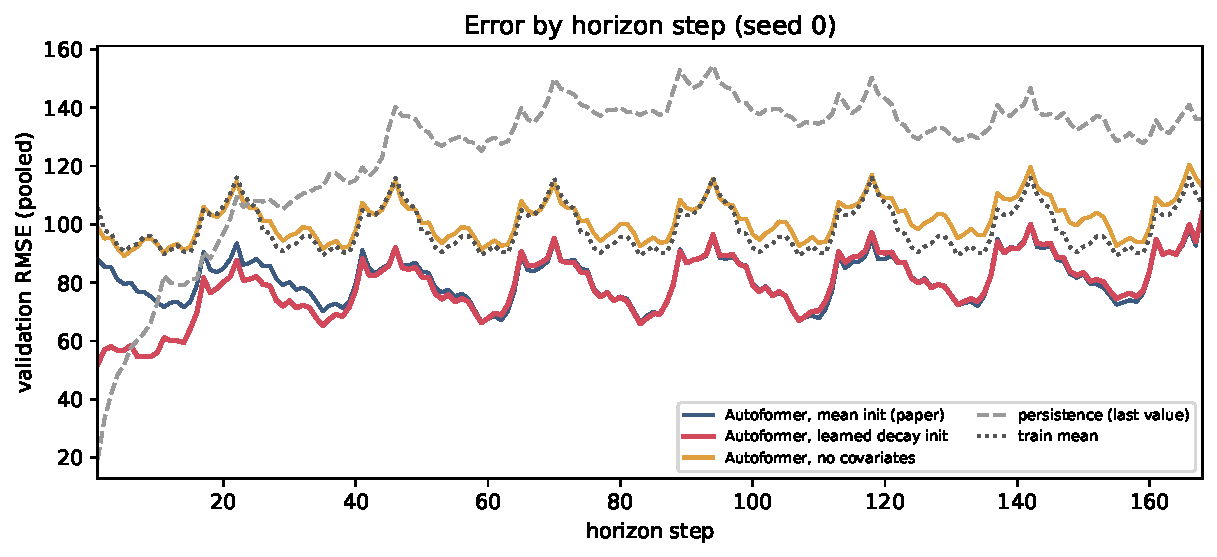
\includegraphics[width=0.8\linewidth]{figures/task2_horizon_curves.pdf}
\caption{Validation RMSE by horizon step (seed 0). The decay initialisation follows persistence early and the mean-initialised model late.}
\label{fig:t2hor}
\end{figure}

\subsection{Final model and leaderboard}
\textbf{Production fit.}
\begin{itemize}
  \item The final model trains on time\_idx 1--41{,}472 and early-stops on the last 13 weeks: RMSE 77.2, block std 27.4 (Fig.~\ref{fig:t2fc}).
  \item It uses seed 0, fixed a priori. $P=6{,}626$; $E=6$ (best epoch 3 plus 3 patience epochs; no refit).
\end{itemize}

\textbf{Leaderboard.} On the hidden week, RMSE is 101.10, MAE 61.40 and sMAPE 53.79\%.
\begin{itemize}
  \item MAE is near the backtest (56.8), and sMAPE is better than it (65.2\%).
  \item RMSE/MAE is 1.65, against about 1.25 in validation, so a few large misses, most likely unforecast pollution-type peaks in a late-December week, dominate the squared error.
  \item One block is a single draw: 101 lies within one standard deviation of the winter-window backtest.
  \item The cost penalty adds only $\approx$0.003 to the score.
\end{itemize}

\begin{figure}[htbp]\centering
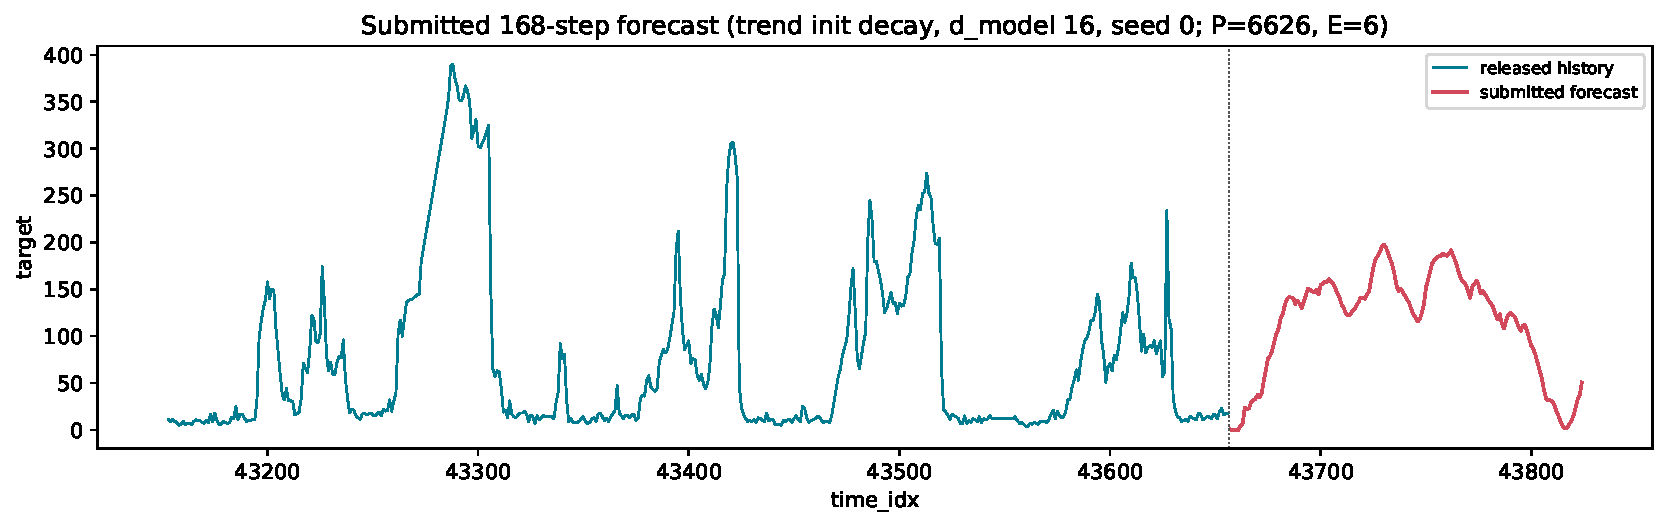
\includegraphics[width=0.85\linewidth]{figures/task2_forecast.pdf}
\caption{Last three weeks of released history and the submitted 168-step forecast.}
\label{fig:t2fc}
\end{figure}

\textbf{Linear reference.} A 78-parameter ridge on the same inputs (last 24 values, future covariates, phase features) reaches validation 62.9 and test 55.3, better than every Autoformer. It is reported for comparison only, since the rules require an Autoformer. The Autoformer passes the ridge's training loss within two epochs while its validation error rises, consistent with~\cite{zeng2023}.

%=====================================================================
\section{Discussion}
\textbf{Inductive bias versus flexibility.} Both tasks give the same answer.
\begin{itemize}
  \item In Task~1, supplying the pace to a linear map beat every learned mixer.
  \item In Task~2, a linear model with the right inputs beat Autoformers with 6--88k parameters.
  \item The largest Autoformer gain came from a one-parameter structural prior (Eq.~\eqref{eq:decay}), not from capacity.
\end{itemize}

\textbf{Agreement with theory.} Confirmed:
\begin{itemize}
  \item the shared-map compromise;
  \item linear amplitude equivariance;
  \item the moving-average leakage of Eq.~\eqref{eq:gain};
  \item recurrence at $P$ and $2P$;
  \item sub-additive switches;
  \item median-like behaviour under a log loss;
  \item the uselessness of past-only covariates under short memory.
\end{itemize}
Deviations, each explained:
\begin{itemize}
  \item Attention's excess held-out loss (overfitting to three stations);
  \item the unsupported prediction in 4(a) (large-range drift is near-linear);
  \item the reference Autoformer's step-1 failure (its decoder initialisation).
\end{itemize}

\textbf{Limitations.}
\begin{itemize}
  \item Task~1 neural results use one data seed.
  \item The width choice relies on an oracle.
  \item Task~2's final model is a single seed, and one leaderboard week is a noisy estimate.
  \item The decay initialisation's benefit on test at $d_{\text{model}}=16$ is not conclusive.
\end{itemize}

%=====================================================================
\section{Conclusion}
\begin{itemize}
  \item On a synthetic benchmark with known structure, a period-routed linear model outperformed Attention and Autoformer-style models on both seen and unseen stations, at a fraction of the cost.
  \item On a real, heavy-tailed series, future-known external variables were the dominant source of skill.
  \item Correcting the Autoformer's decoder initialisation with a theory-derived, one-parameter prior improved it consistently.
\end{itemize}
Choosing the right assumptions mattered more than adding flexibility.

%=====================================================================
\begin{thebibliography}{9}
\bibitem{wu2021} H.~Wu, J.~Xu, J.~Wang, and M.~Long, ``Autoformer: Decomposition transformers with auto-correlation for long-term series forecasting,'' in \emph{Proc.\ NeurIPS}, 2021.
\bibitem{vaswani2017} A.~Vaswani \emph{et al.}, ``Attention is all you need,'' in \emph{Proc.\ NeurIPS}, 2017.
\bibitem{zeng2023} A.~Zeng, M.~Chen, L.~Zhang, and Q.~Xu, ``Are transformers effective for time series forecasting?'' in \emph{Proc.\ AAAI}, 2023.
\bibitem{hyndman} R.~J.~Hyndman and G.~Athanasopoulos, \emph{Forecasting: Principles and Practice}, 3rd ed., OTexts, \S5.10.
\bibitem{cleveland1990} R.~B.~Cleveland, W.~S.~Cleveland, J.~E.~McRae, and I.~Terpenning, ``STL: A seasonal-trend decomposition procedure based on loess,'' \emph{J.\ Official Statistics}, vol.~6, no.~1, pp.~3--73, 1990.
\end{thebibliography}

%=====================================================================
\appendix
\section{Generative-AI Use}\label{app:ai}
Generative AI (Claude, Anthropic, via Claude Code) was used as the course policy permits. The table lists each prompt with a summary of the output.

\begin{center}\footnotesize
\begin{tabularx}{\linewidth}{>{\raggedright\arraybackslash}p{3.3cm}X}
\toprule
Prompt (verbatim) & Output (summary)\\
\midrule
``can you have a look at the assignemnt and audit the code attached with the email, please make two task in very professional way under their own sub folders'' & Repository structure. Task~1 cells and the full-preset run. Harness audit. Autoformer, pipeline, multi-seed study, forecast.\\
``can you have a llook if the results are as they were expected and if these results are in line with the theory'' & Theory checks; extra Task~1 seeds; the per-horizon diagnosis.\\
``is there any ways to deal with the issues \ldots{} the remedy should be allowed and with in the limits'' & Learned decay initialisation (5 seeds). Ensemble and linear skip branch not used.\\
``can you make an explainer document in latex format \ldots'' & A separate study guide.\\
Questions on results, metrics, $P$/$E$ & Explanations; detection of the declared-$P$ mismatch.\\
``can you make the final report now follow the guidelines \ldots''; ``you have to made the report like we do for the paper'' & This paper. Responses 1A and 4(a) derive expectations from model assumptions; 4(a) is tested.\\
\bottomrule
\end{tabularx}
\end{center}

\textbf{Edits made.} I reviewed and verified the code, the experimental results and this report. Specifically, I re-ran the notebook checks and compared the reported numbers with the exported Outputs and result files. No substantive edits were made to the AI outputs.

\section{Reflection Questions (Q2.1--Q2.9)}
\textbf{Q2.1.} Auto-Correlation suits a stable dominant period, as in Task~1. It discards point-wise, event-like dependencies, which dominate this weather-driven series. A drifting period misaligns fixed delays.

\textbf{Q2.2.} A moving average assumes a locally linear trend: it flattens trends near edges, shaves curvature, and smears level shifts. STL follows curvature, at the cost of extra hyperparameters.

\textbf{Q2.3.} Repeated decomposition stops trend re-entering after each nonlinearity. It hurts when the level is the signal: here it hid the ``start from now'' information (Section~\ref{sec:hor}).

\textbf{Q2.4.} Small $k$ misses harmonics; large $k$ admits noise delays. $\ln L$ is a convenient budget, and $k$ should track the number of true periodicities. $c=1$ vs 3 did not matter here.

\textbf{Q2.5.} One-shot forecasting avoids compounding errors and exposure bias, but must learn continuity at the boundary. Recursive forecasting keeps continuity but accumulates correlated errors as $H$ grows.

\textbf{Q2.6.} Window normalisation discards level, which matters when dynamics depend on it (mean reversion). Hence anchoring alone did not help here, although it suits Task~1's offset differences.

\textbf{Q2.7.} Known-future covariates belong in the decoder's horizon; past-only ones in the encoder. Future wind is informative, origin-time wind nearly useless (Table~\ref{tab:exog}), and deterministic phase features help in both regimes.

\textbf{Q2.8.} Without timestamps there are no calendar features. Periods were recovered from the periodogram, assuming uniform sampling and stable periods.

\textbf{Q2.9.} Structural models win on short, regular, high signal-to-noise series. This long but noisy, heavy-tailed, weakly periodic series still favoured a 78-parameter linear model. A strong linear baseline on validation is the practical pre-training test.

\end{document}
